%%
%% Automatically generated file from DocOnce source
%% (https://github.com/hplgit/doconce/)
%%

% #define PREAMBLE

% #ifdef PREAMBLE
%-------------------- begin preamble ----------------------

\documentclass[%
oneside,                 % oneside: electronic viewing, twoside: printing
final,                   % draft: marks overfull hboxes, figures with paths
10pt,french]{article}

\listfiles               %  print all files needed to compile this document

\usepackage{relsize,makeidx,color,setspace,amsmath,amsfonts,amssymb}
\usepackage[table]{xcolor}
\usepackage{bm,ltablex,microtype}

\usepackage[pdftex]{graphicx}

% Packages for typesetting blocks of computer code
\usepackage{fancyvrb,framed,moreverb}

% Define colors
\definecolor{orange}{cmyk}{0,0.4,0.8,0.2}
\definecolor{tucorange}{rgb}{1.0,0.64,0}
\definecolor{darkorange}{rgb}{.71,0.21,0.01}
\definecolor{darkgreen}{rgb}{.12,.54,.11}
\definecolor{myteal}{rgb}{.26, .44, .56}
\definecolor{gray}{gray}{0.45}
\definecolor{mediumgray}{gray}{.8}
\definecolor{lightgray}{gray}{.95}
\definecolor{brown}{rgb}{0.54,0.27,0.07}
\definecolor{purple}{rgb}{0.5,0.0,0.5}
\definecolor{darkgray}{gray}{0.25}
\definecolor{darkblue}{rgb}{0,0.08,0.45}
\definecolor{darkblue2}{rgb}{0,0,0.8}
\definecolor{lightred}{rgb}{1.0,0.39,0.28}
\definecolor{lightgreen}{rgb}{0.48,0.99,0.0}
\definecolor{lightblue}{rgb}{0.53,0.81,0.92}
\definecolor{lightblue2}{rgb}{0.3,0.3,1.0}
\definecolor{lightpurple}{rgb}{0.87,0.63,0.87}
\definecolor{lightcyan}{rgb}{0.5,1.0,0.83}

\colorlet{comment_green}{green!50!black}
\colorlet{string_red}{red!60!black}
\colorlet{keyword_pink}{magenta!70!black}
\colorlet{indendifier_green}{green!70!white}

% Backgrounds for code
\definecolor{cbg_gray}{rgb}{.95, .95, .95}
\definecolor{bar_gray}{rgb}{.92, .92, .92}

\definecolor{cbg_yellowgray}{rgb}{.95, .95, .85}
\definecolor{bar_yellowgray}{rgb}{.95, .95, .65}

\colorlet{cbg_yellow2}{yellow!10}
\colorlet{bar_yellow2}{yellow!20}

\definecolor{cbg_yellow1}{rgb}{.98, .98, 0.8}
\definecolor{bar_yellow1}{rgb}{.98, .98, 0.4}

\definecolor{cbg_red1}{rgb}{1, 0.85, 0.85}
\definecolor{bar_red1}{rgb}{1, 0.75, 0.85}

\definecolor{cbg_blue1}{rgb}{0.87843, 0.95686, 1.0}
\definecolor{bar_blue1}{rgb}{0.7,     0.95686, 1}

%\setlength{\fboxsep}{-1.5mm}  % adjust cod_vpad/pro_vpad background box

%% Background for code blocks (parameter is color name)

%% pro/cod_vpad: gives some vertical padding before and after the text
%% (but has more simplistic code than _cod/pro_tight+cod/pro).
%% pro/cod_vpad can be used to enclose Verbatim or lst begin/end for code.
%% pro/cod calls _pro/cod_tight and has very little vertical padding,
%% used to enclose Verbatim and other begin/end for code.
%% (pro/cod is what the ptex2tex program could produce with the
%% Blue/BlueBar definitions in .ptex2tex.cfg.)

\newenvironment{cod_vpad}[1]{
   \def\FrameCommand{\colorbox{#1}}
   \MakeFramed{\FrameRestore}}
   {\endMakeFramed}

\newenvironment{_cod_tight}[1]{
   \def\FrameCommand{\colorbox{#1}}
   \FrameRule0.6pt\MakeFramed {\FrameRestore}\vskip3mm}
   {\vskip0mm\endMakeFramed}

\newenvironment{cod}[1]{
\bgroup\rmfamily
\fboxsep=0mm\relax
\begin{_cod_tight}{#1}
\list{}{\parsep=-2mm\parskip=0mm\topsep=0pt\leftmargin=2mm
\rightmargin=2\leftmargin\leftmargin=4pt\relax}
\item\relax}
{\endlist\end{_cod_tight}\egroup}

%% Background for complete program blocks (parameter 1 is color name
%% for background, parameter 2 is color for left bar)
\newenvironment{pro_vpad}[2]{
   \def\FrameCommand{\color{#2}\vrule width 1mm\normalcolor\colorbox{#1}}
   \MakeFramed{\FrameRestore}}
   {\endMakeFramed}

\newenvironment{_pro_tight}[2]{
   \def\FrameCommand{\color{#2}\vrule width 1mm\normalcolor\colorbox{#1}}
   \FrameRule0.6pt\MakeFramed {\advance\hsize-2mm\FrameRestore}\vskip3mm}
   {\vskip0mm\endMakeFramed}

\newenvironment{pro}[2]{
\bgroup\rmfamily
\fboxsep=0mm\relax
\begin{_pro_tight}{#1}{#2}
\list{}{\parsep=-2mm\parskip=0mm\topsep=0pt\leftmargin=2mm
\rightmargin=2\leftmargin\leftmargin=4pt\relax}
\item\relax}
{\endlist\end{_pro_tight}\egroup}

\usepackage{minted}
\usemintedstyle{default}

\usepackage[T1]{fontenc}
%\usepackage[latin1]{inputenc}
\usepackage{ucs}
\usepackage[utf8x]{inputenc}

\usepackage{lmodern}         % Latin Modern fonts derived from Computer Modern

% Hyperlinks in PDF:
\definecolor{linkcolor}{rgb}{0,0,0.4}
\usepackage{hyperref}
\hypersetup{
    breaklinks=true,
    colorlinks=true,
    linkcolor=linkcolor,
    urlcolor=linkcolor,
    citecolor=black,
    filecolor=black,
    %filecolor=blue,
    pdfmenubar=true,
    pdftoolbar=true,
    bookmarksdepth=3   % Uncomment (and tweak) for PDF bookmarks with more levels than the TOC
    }
%\hyperbaseurl{}   % hyperlinks are relative to this root

\setcounter{tocdepth}{2}  % levels in table of contents

% Tricks for having figures close to where they are defined:
% 1. define less restrictive rules for where to put figures
\setcounter{topnumber}{2}
\setcounter{bottomnumber}{2}
\setcounter{totalnumber}{4}
\renewcommand{\topfraction}{0.95}
\renewcommand{\bottomfraction}{0.95}
\renewcommand{\textfraction}{0}
\renewcommand{\floatpagefraction}{0.75}
% floatpagefraction must always be less than topfraction!
% 2. ensure all figures are flushed before next section
\usepackage[section]{placeins}
% 3. enable begin{figure}[H] (often leads to ugly pagebreaks)
%\usepackage{float}\restylefloat{figure}

% prevent orhpans and widows
\clubpenalty = 10000
\widowpenalty = 10000

\newenvironment{doconceexercise}{}{}
\newcounter{doconceexercisecounter}


% ------ header in subexercises ------
%\newcommand{\subex}[1]{\paragraph{#1}}
%\newcommand{\subex}[1]{\par\vspace{1.7mm}\noindent{\bf #1}\ \ }
\makeatletter
% 1.5ex is the spacing above the header, 0.5em the spacing after subex title
\newcommand\subex{\@startsection{paragraph}{4}{\z@}%
                  {1.5ex\@plus1ex \@minus.2ex}%
                  {-0.5em}%
                  {\normalfont\normalsize\bfseries}}
\makeatother


% --- end of standard preamble for documents ---


\usepackage[french]{babel}

% insert custom LaTeX commands...

\raggedbottom
\makeindex
\usepackage[totoc]{idxlayout}   % for index in the toc
\usepackage[nottoc]{tocbibind}  % for references/bibliography in the toc

%-------------------- end preamble ----------------------

\begin{document}

% matching end for #ifdef PREAMBLE
% #endif

\newcommand{\exercisesection}[1]{\subsection*{#1}}


% ------------------- main content ----------------------

% TITLE: TP 3: Introduction à matplotlib et numpy
% AUTHOR: Ahmed Ammar {copyright|CC BY} Email:ahmed.ammar@fst.utm.tn at Université de Tunis El Manar.
% DATE: Mercredi, 5 décembre 2018
% 
% TOC: on

% !split


% --- begin exercise ---
\begin{doconceexercise}
\refstepcounter{doconceexercisecounter}

\exercisesection{Exercise \thedoconceexercisecounter: Tracer une fonction}


Ecrivez un programme qui trace la fonction $g(y) = e^{-y} sin(4y)$ pour $y \in [0, 4]$ en utilisant une ligne continue rouge. Utilisez 500 intervalles pour évaluer les points dans [0,4]. Stockez toutes les coordonnées et les valeurs dans des tableaux. Placez le texte des graduations sur les axes et utilisez le titre "Onde sinusoïdale atténuée".


% --- begin solution of exercise ---
\paragraph{Solution.}
La programme qui trace la fonction $g(y)$ est:
\begin{cod}{cbg_gray}\begin{minted}[fontsize=\fontsize{9pt}{9pt},linenos=false,mathescape,baselinestretch=1.0,fontfamily=tt,xleftmargin=2mm]{python}
# Importer tout de matplotlib et numpy
from pylab import *

def g(y):
    return exp(-y)*sin(4*y)

y = np.linspace(0, 4, 501)
# définir un nouveau graphique
plt.figure()
# tracer la fonction g(y) avec ligne solide rouge
plt.plot(y, g(y), 'r-')
plt.xlabel('y'); plt.ylabel('g(y)')
plt.title('Onde sinusoïdale atténuée')
 # sauvgarder le grahique (format PNG et PDF)
plt.savefig("fig_ex1.png"); plt.savefig("fig_ex1.pdf")
# Afficher le graphique
plt.show()
\end{minted}
\end{cod}
\noindent

% --- end solution of exercise ---

\end{doconceexercise}
% --- end exercise ---




% --- begin exercise ---
\begin{doconceexercise}
\refstepcounter{doconceexercisecounter}

\exercisesection{Exercise \thedoconceexercisecounter: Tracer deux fonctions}


Comme Exercice 1, mais ajouter une courbe en pointillé noir pour la fonction $h(y) = e^{-\frac{3}{2}y} sin(4y)$. Inclure une légende pour chaque courbe (avec les noms $g$ et $h$).


% --- begin solution of exercise ---
\paragraph{Solution.}
La programme qui trace la fonction $g(y)$ avec une nouvelle fonction $h(y)$ est:
\begin{cod}{cbg_gray}\begin{minted}[fontsize=\fontsize{9pt}{9pt},linenos=false,mathescape,baselinestretch=1.0,fontfamily=tt,xleftmargin=2mm]{python}
# Importer tout de matplotlib et numpy
from pylab import *

def g(y):
    return exp(-y)*sin(4*y)

def h(y):
    return exp(-(3./2)*y)*sin(4*y)

y = np.linspace(0, 4, 501)
plt.figure()
plt.plot(y, g(y), 'r-', y, h(y), 'k--')
plt.xlabel('y'); plt.ylabel('g(y)')
plt.title('Onde sinusoïdale atténuée')
plt.legend(['g', 'h'])

plt.savefig("fig_ex2.png"); plt.savefig("fig_ex2.pdf")
plt.show()
\end{minted}
\end{cod}
\noindent

% --- end solution of exercise ---

\end{doconceexercise}
% --- end exercise ---




% --- begin exercise ---
\begin{doconceexercise}
\refstepcounter{doconceexercisecounter}

\exercisesection{Exercise \thedoconceexercisecounter: Racines d’une équation du second degré}


Dans l'"application de l'exercice 4 dans le TP3, nous avons montré la représentation graphique d'une équation du second degré $f(x)=0.83x^2+3.8x+2.48$ ainsi que ses racines réelles:



\vspace{6mm}

% inline figure
\centerline{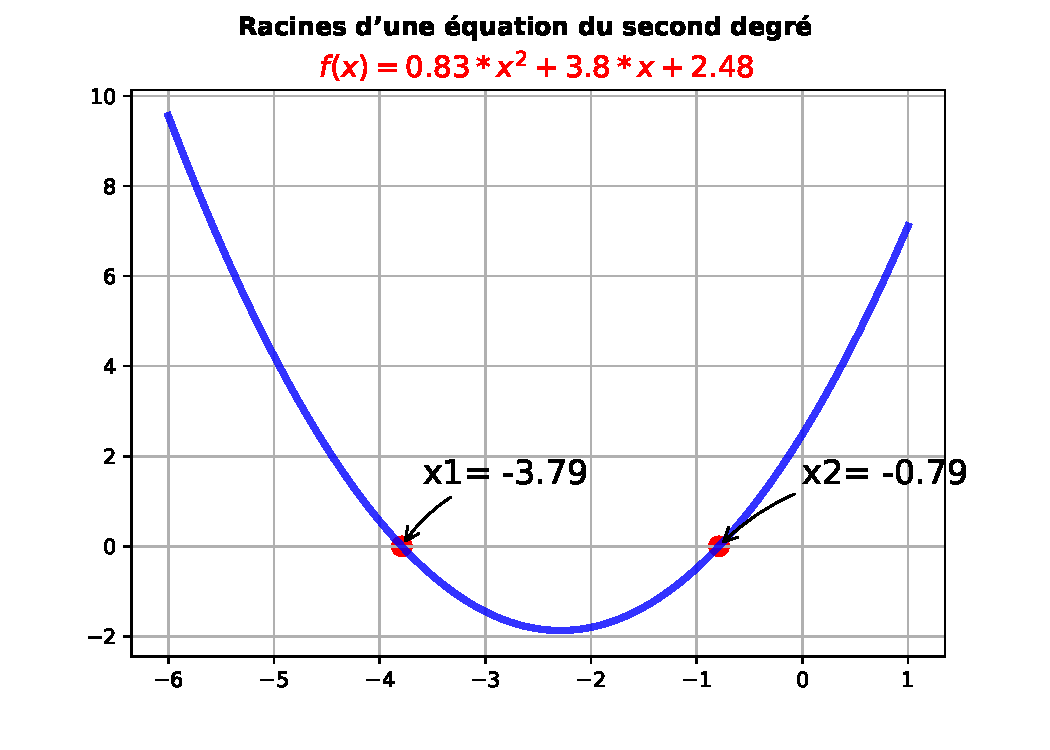
\includegraphics[width=0.7\linewidth]{figs/equation2deg.pdf}}

\vspace{6mm}


Reproduire ce graphique en utilisant la fonction \texttt{EqSecondDegree(a,b,c)} du script Python \texttt{racines.py} pour déterminer les valeurs des racines x1 et x2 de l’équation $f(x)$.


% --- begin solution of exercise ---
\paragraph{Solution.}
Le programme qui reproduit la figure en utilisant la fonction \texttt{EqSecondDegree()}:

\begin{cod}{cbg_gray}\begin{minted}[fontsize=\fontsize{9pt}{9pt},linenos=false,mathescape,baselinestretch=1.0,fontfamily=tt,xleftmargin=2mm]{python}

from pylab import *
from racines import EqSecondDegree
# NOTE: le module racines est le fichier racines.py
# qu'on doit placer dans le répertoire de travail.

def f(x):
    return 0.83 * x**2 + 3.8 * x + 2.48
x = linspace(-6, 1, 200)
y = f(x)
x1, x2 = EqSecondDegree(0.83, 3.8, 2.48)

figure(figsize=(7, 5), dpi=80)
plot(x, y, color="blue", linewidth=3, linestyle="-", alpha=.8)
scatter([x1,x2], [f(x1), f(x2)], 80, color='red')

annotate('x1= {:.2f}'.format(x1),
             xy=(x1, f(x1)), xycoords='data',
             xytext=(+10, +30), textcoords='offset points', fontsize=16,
             arrowprops=dict(arrowstyle="->", connectionstyle="arc3,rad=.2"))
annotate('x2= {:.2f}'.format(x2),
             xy=(x2, f(x2)), xycoords='data',
             xytext=(+40, +30), textcoords='offset points', fontsize=16,
             arrowprops=dict(arrowstyle="->", connectionstyle="arc3,rad=.2"))

suptitle("Racines d’une équation du second degré", fontweight= 'bold')
title(r"$f(x) = 0.83 * x^2 + 3.8 * x + 2.48$",fontsize=14, color = 'b')

plt.grid()

plt.savefig("equation2deg.png"); plt.savefig("equation2deg.pdf")
plt.show()
\end{minted}
\end{cod}
\noindent

% --- end solution of exercise ---

\end{doconceexercise}
% --- end exercise ---




% --- begin exercise ---
\begin{doconceexercise}
\refstepcounter{doconceexercisecounter}

\exercisesection{Exercise \thedoconceexercisecounter: Loi de Snell-Descartes pour la réfraction}


La loi de Snell-Descartes stipule que le rapport sinus de l'angle d'incidence sur le sinus de l'angle de réfraction est équivalent au rapport de la vitesse de phase dans le premier milieu à la vitesse de phase dans le deuxième milieu, ou équivalent à l'inverse du rapport des indices de réfraction.

$$\dfrac{\sin\theta_1}{\sin\theta_2} = \dfrac{v_1}{v_2} = \dfrac{n_2}{n_1}$$

Où $\theta_1$ est l'angle d'incidence dans le premier milieu, $\theta_2$ est l'angle de réfraction dans le deuxième milieu, tous les angles mesurés à partir de la normale de la frontière (dioptre), $v_1$ et $v_2$ sont respectivement les vitesses dans les deux milieux, et $n_1$ et $n_2$ sont les indices de réfraction du premier et du deuxième milieux, respectivement.



\vspace{6mm}

% inline figure
\centerline{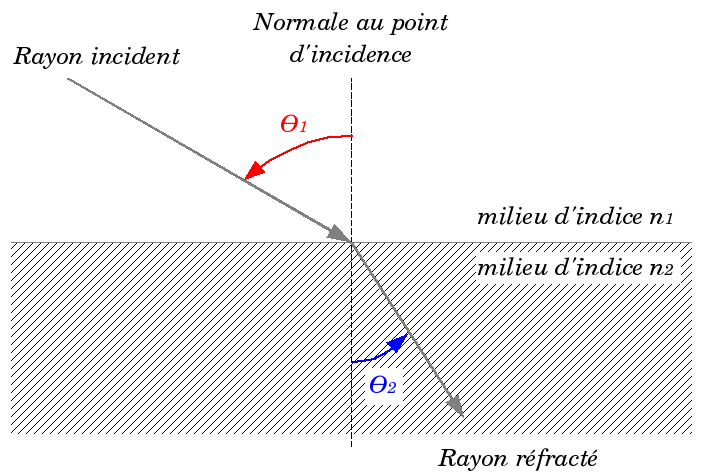
\includegraphics[width=0.7\linewidth]{figs/Refraction_fr.png}}

\vspace{6mm}



\textbf{Objectif:}

Ecrire un programme Python pour tracer angle de réfraction en fonction de l'angle d'incidence.

\textbf{Algorithme:}
\begin{itemize}
 \item Afficher: \texttt{"Loi de Snell-Descartes pour la réfraction."}

 \item Demender un nombre réel n1: \texttt{"Entrez l'indice de réfraction du premier milieu: "}

 \item Demender un nombre réel n2: \texttt{"Entrez l'indice de réfraction du deuxième milieu: "}

 \item choix = 'o' et compteur k = 0

 \item Tant que choix == 'o':
\begin{itemize}

   \item Stoker dans une liste theta1 un nombre réel \texttt{theta1[k]}: \texttt{"Entrez l'angle d'incidence en degrés: "}

   \item Condition: \texttt{si (n1*sin(theta1[k]))/n2 < -1 ou n1 * (n1*sin(theta1[k]))/n2 > 1}:
\begin{itemize}

     \item Afficher: \texttt{"Il y aura une réflexion totale pour l'angle d'incidence donné. Essayez d'autres valeurs."}

     \item Stoker dans une liste theta1 un nombre réel \texttt{theta1[k]}: \texttt{"Entrez l'angle d'incidence en degrés: "}

\end{itemize}

\noindent
   \item Stoker dans la liste la valeur \texttt{theta2[k]}: \texttt{arcsin(n1*sin(theta1[k])/n2}

   \item Afficher: \texttt{"L'angle d'incidence est de theta1[k] degrés et l'angle de réfraction de theta2[k] degrés."}

   \item Entrer une nouvelle valeur de choix: \texttt{"Voulez-vous entrer plus de valeurs (o / n)?: "}

   \item k+=1

\end{itemize}

\noindent
 \item si choix == 'n':
\begin{itemize}

   \item Tracer le graphique de theta2 en fonction de theta1 (exemple pour 3 valeurs de theta1):
\end{itemize}

\noindent
\end{itemize}

\noindent
\vspace{6mm}

% inline figure
\centerline{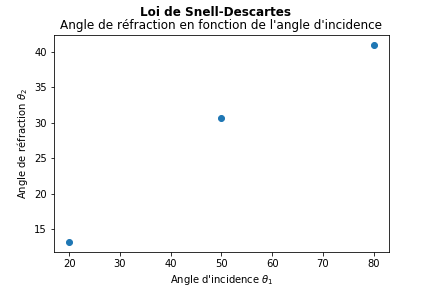
\includegraphics[width=0.7\linewidth]{figs/snell.png}}

\vspace{6mm}




% --- begin solution of exercise ---
\paragraph{Solution.}
Le code Python qui traduit l'algorithme précédent est:
\begin{cod}{cbg_gray}\begin{minted}[fontsize=\fontsize{9pt}{9pt},linenos=false,mathescape,baselinestretch=1.0,fontfamily=tt,xleftmargin=2mm]{python}
from pylab import *

print("Loi de Snell-Descartes pour la réfraction.")
n1 = float(input("Entrez l'indice de réfraction du premier milieu: "))
n2 = float(input("Entrez l'indice de réfraction du deuxième milieu: "))
choix = "o"
k = 0
theta1, theta2 = [],[]
while choix == "o":
    theta1.append(float(input("Entrez l'angle d'incidence en degrés: ")))
    if (n1*sin(deg2rad(theta1[k])))/n2 < -1 or n1 * (n1*sin(deg2rad(theta1[k])))/n2 > 1:
        print("Il y aura une réflexion totale pour l'angle d'incidence donné. Essayez d'autres valeurs.")
        theta1.append(float(input("Entrez l'angle d'incidence en degrés: ")))
    theta2.append(rad2deg(arcsin(n1*sin(deg2rad(theta1[k]))/n2)))
    print("L'angle d'incidence est de {:.2f} degrés et l'angle de réfraction de {:.2f} degrés.".format(theta1[k], theta2[k]))
    choix = input("Voulez-vous entrer plus de valeurs (o / n)?: ")
    while (choix!='o') and (choix!='n'):
        print("Entrée invalide. Tapez o ou n. ")
        choix = input("Voulez-vous entrer plus de valeurs (o / n)?: ")

    k +=1

if choix == "n":
    scatter(theta1, theta2)
    suptitle("Loi de Snell-Descartes", fontweight='bold')
    title("Angle de réfraction en fonction de l'angle d'incidence")
    xlabel("Angle d'incidence" + r" $\theta_1$")
    ylabel("Angle de réfraction" + r" $\theta_2$")
    savefig("snell.png")
    show()
\end{minted}
\end{cod}
\noindent

% --- end solution of exercise ---

\end{doconceexercise}
% --- end exercise ---




% --- begin exercise ---
\begin{doconceexercise}
\refstepcounter{doconceexercisecounter}

\exercisesection{Exercise \thedoconceexercisecounter: Diffraction par une ouverture rectangulaire}




\vspace{6mm}

% inline figure
\centerline{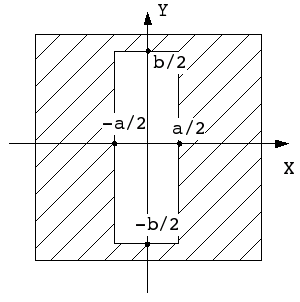
\includegraphics[width=0.7\linewidth]{figs/Diffr_ouv_rectangle.png}}

\vspace{6mm}



Une ouverture rectangulaire de côtés a et b correspond à une transmission $t(X, Y)$ définie par :
\[ \left\{
\begin{array}{ll}
t(X,Y) = 1 & si \ |X|<a/2 \ et \ |Y|<b/2 \\
t(X,Y) = 0 & sinon
\end{array}
\right. \]
Le calcul de l'intensité diffractée par une telle ouverture, c’est-à-dire du carré du module de l'amplitude E(M), donne :
$$I(x,y)=|E(x,y)|^2=I_0 \  \mathrm{sinc}^2\left(\frac{\pi xa}{\lambda f_2}\right) \mathrm{sinc}^2\left(\frac{\pi yb}{\lambda f_2}\right)$$



\vspace{6mm}

% inline figure
\centerline{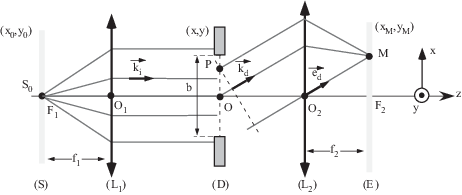
\includegraphics[width=0.7\linewidth]{figs/figDiff.png}}

\vspace{6mm}



les dimensions de la tache centrale sont :
\begin{itemize}
 \item $\Delta x = 2 \lambda f_2/a $

 \item $\Delta y = 2 \lambda f_2/b $
\end{itemize}

\noindent
\textbf{Le programme Python:}


\subex{a)}
Écrire une fonction \Verb!Intensity(X, Y, a = 0.2 * 1.E-3, b = 0.2 * 1.E-3, lambda_ = 630 * 1.E-9, f2 = 10)! qui affiche les dimensions de la tache centrale ($\Delta x$ et $\Delta y$) et retourne la valeur de $I(X,Y)$. Avec:
\begin{itemize}
\item \texttt{X} et \texttt{Y} sont respectivement l'abscisse et l'ordonnée à l'écran.

\item \texttt{a} la largeur de la fente (par défaut = 0.2 mm)

\item \texttt{b} la hauteur de la fente (par défaut = 0.2 mm)

\item \Verb!lambda_! la longueur d'onde de la lumière incidente (par défaut = 630 nm)

\item \texttt{f2} la distance fente - écran (par défaut = 10 m)
\end{itemize}

\noindent
On considère que $I_0 = 1$ par convention.


% --- begin solution of exercise ---
\paragraph{Solution.}
la fonction \texttt{Intensity()} s'écrit:

\begin{cod}{cbg_gray}\begin{minted}[fontsize=\fontsize{9pt}{9pt},linenos=false,mathescape,baselinestretch=1.0,fontfamily=tt,xleftmargin=2mm]{python}
from pylab import *

def Intensity(X, Y, a = 0.2 * 1.E-3, b = 0.2 * 1.E-3, lambda_ = 630 * 1.E-9, f2 = 10):
    # les dimensions de la tache centrale
    Dx = 1.E2 * (2 * lambda_ * f2) / a
    print("La largeur du maximum central le long (Ox) = {:.3f} cm".format(Dx))
    Dy = 1.E2 * (2 * lambda_ * f2) / b
    print("La largeur du maximum central le long (Oy) = {:.3f} cm".format(Dy))
    # Variables intermidières
    A = (pi * X * a)/(lambda_ * f2)
    B = (pi * Y * b)/(lambda_ * f2)
    return (sin(A)/A)**2 * (sin(B)/B)**2
\end{minted}
\end{cod}
\noindent

% --- end solution of exercise ---

\subex{b)}
Créez le graphique de diffraction suivant (à l'aide de la fonction \href{{https://codetunisia.github.io/CoursSimNum/cours3/md/cours3.html#image-pixelis%C3%A9e}}{\nolinkurl{imshow()}}) pour un écran de 30/30 cm:


\vspace{6mm}

% inline figure
\centerline{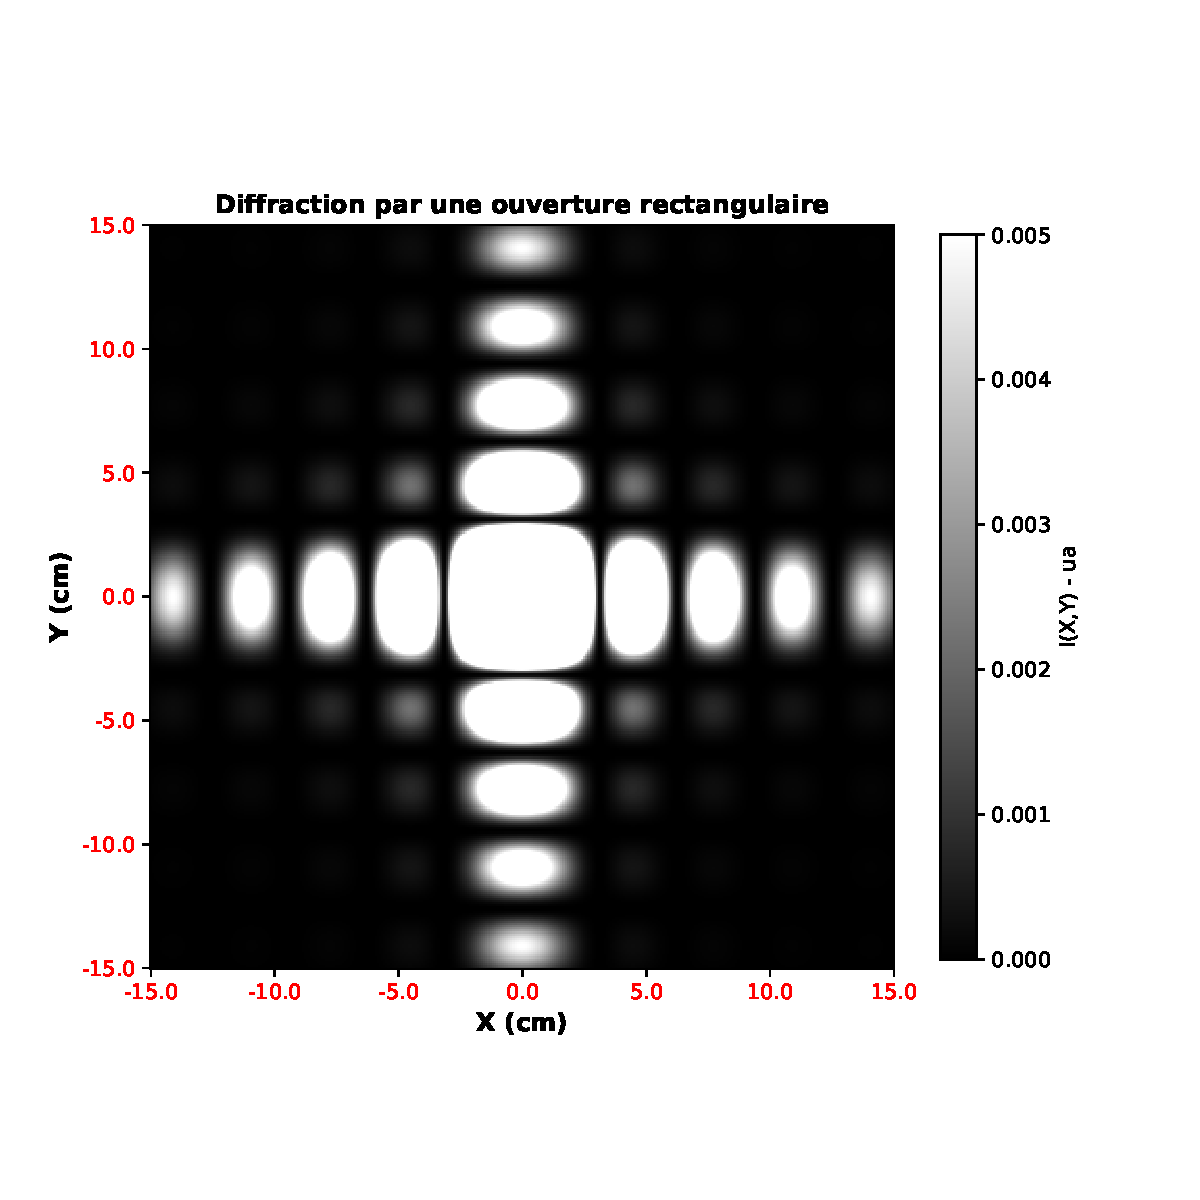
\includegraphics[width=0.7\linewidth]{figs/diff2D.pdf}}

\vspace{6mm}




% --- begin solution of exercise ---
\paragraph{Solution.}
La représentation graphique de la figure de diffraction en 2D:
\begin{cod}{cbg_gray}\begin{minted}[fontsize=\fontsize{9pt}{9pt},linenos=false,mathescape,baselinestretch=1.0,fontfamily=tt,xleftmargin=2mm]{python}
# coordonnées de l'écran
X, Y = meshgrid(linspace(-15*1e-2, 15*1e-2, 400), linspace(-15*1e-2, 15*1e-2, 400))
# Intensité
I = Intensity(X, Y)
# Figure de diffraction
fig, ax = plt.subplots(figsize=(8,8))
im = imshow(I, cmap='gray', interpolation='bilinear',
                origin='lower',  vmin= 0, vmax = 0.005)
cb = fig.colorbar(im, label="I(X,Y) - ua", shrink=0.8)
title('Diffraction par une ouverture rectangulaire', fontweight='bold')

xlabel('X (cm)', fontsize=12, fontweight='bold')
ylabel('Y (cm)', fontsize=12, fontweight='bold')
xticks(linspace(0, 400, 7))
ax.set_xticklabels(linspace(-15, 15, 7),  color='r')
yticks(linspace(0, 400, 7))
ax.set_yticklabels(linspace(-15, 15, 7),  color='r')

savefig("diff2D.png"); savefig("diff2D.pdf")
show()
\end{minted}
\end{cod}
\noindent

% --- end solution of exercise ---

\subex{c)}
Créez le graphique 3D de diffraction suivant (voir la partie \href{{https://codetunisia.github.io/CoursSimNum/cours3/md/cours3.html#trac%C3%A9-de-surfaces}}{tracé de surfaces} du cours):


\vspace{6mm}

% inline figure
\centerline{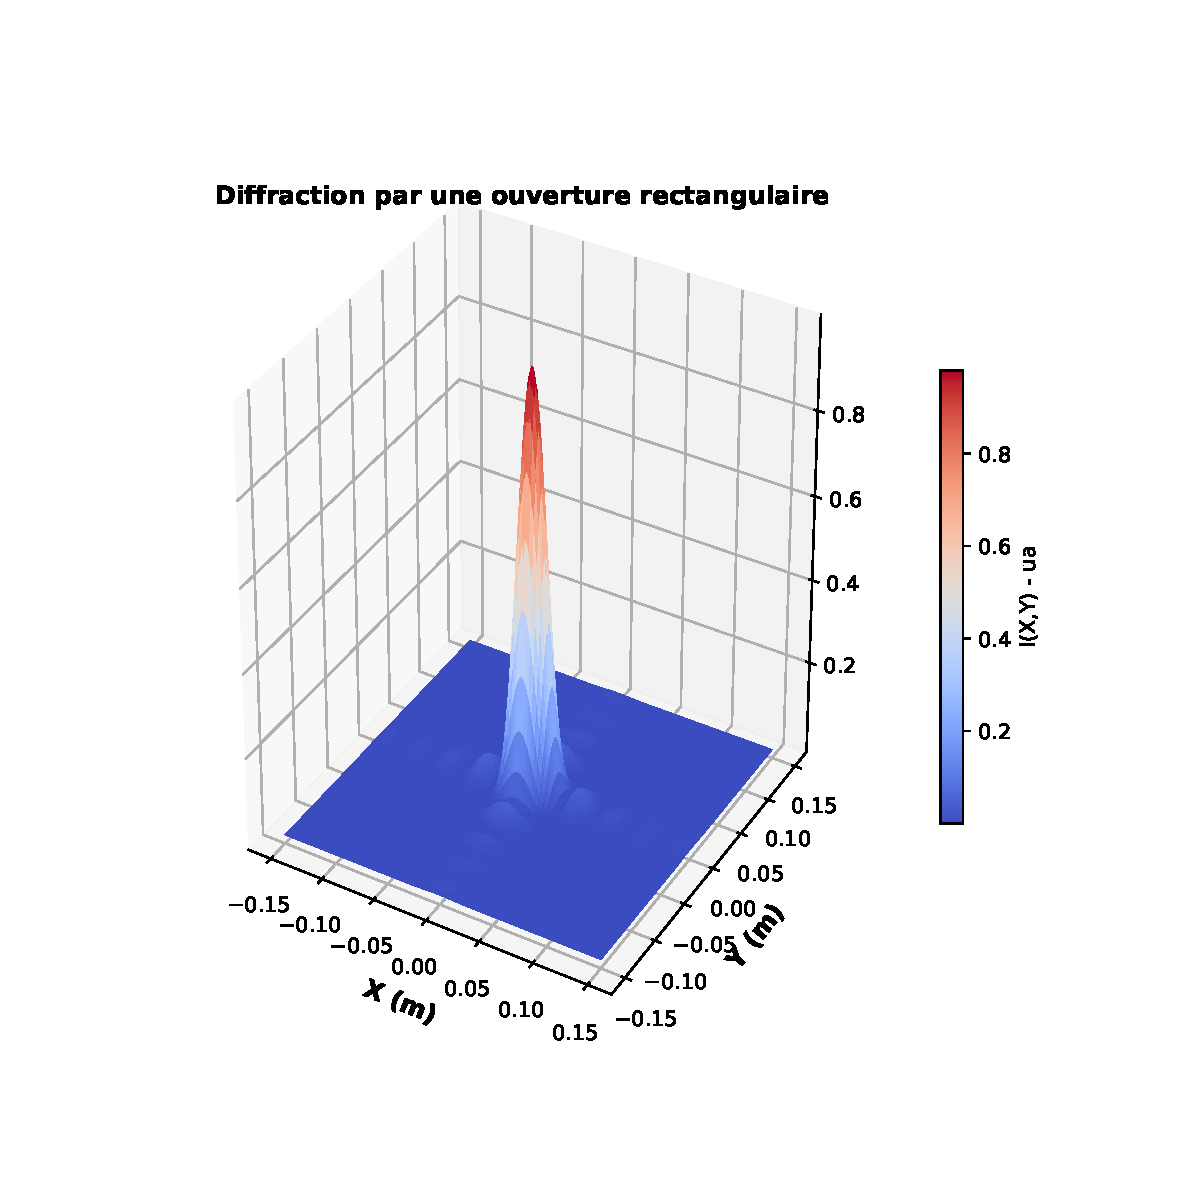
\includegraphics[width=0.7\linewidth]{figs/diff3D.pdf}}

\vspace{6mm}




% --- begin solution of exercise ---
\paragraph{Solution.}
La représentation graphique de la figure de diffraction en 3D:

\begin{cod}{cbg_gray}\begin{minted}[fontsize=\fontsize{9pt}{9pt},linenos=false,mathescape,baselinestretch=1.0,fontfamily=tt,xleftmargin=2mm]{python}
# coordonnées de l'écran
X, Y = meshgrid(linspace(-15*1e-2, 15*1e-2, 400), linspace(-15*1e-2, 15*1e-2, 400))
# Intensité
I = Intensity(X, Y)

# Figure de diffraction
fig = plt.figure(figsize=(8,8))
ax = plt.axes(projection='3d')
# plot surface
p = ax.plot_surface(X, Y, I, rstride=4, cstride=4, cmap='coolwarm',
                    linewidth=0, antialiased=False)
cb = fig.colorbar(p, label="I(X,Y) - ua", shrink=0.5)

xlabel('X (m)', fontsize=12, fontweight='bold')
ylabel('Y (m)', fontsize=12, fontweight='bold')
title('Diffraction par une ouverture rectangulaire', fontweight='bold')

savefig("diff3D.png"); savefig("diff3D.pdf")
plt.show()
\end{minted}
\end{cod}
\noindent

% --- end solution of exercise ---

\end{doconceexercise}
% --- end exercise ---


% !split


% --- begin exercise ---
\begin{doconceexercise}
\refstepcounter{doconceexercisecounter}

\exercisesection{Exercise \thedoconceexercisecounter: Tracer un graphique à partir d'un fichier (données satellitaires)}


Les mesures de flux de rayons X du satellite GOES (\href{{https://fr.wikipedia.org/wiki/Geostationary_Operational_Environmental_Satellite}}{Geostationary Operational Environmental Satellite}) ont été effectuées depuis 1974. Le graphique à rayons X GOES (flux de 1 à 8 angströms) faisant l’objet de cet exercice peut suivre l’activité solaire et les éruptions solaires. De grandes éruptions de rayons X solaires peuvent modifier l'ionosphère terrestre et bloquer les transmissions radio haute fréquence (HF) du côté de la Terre éclairé par le soleil.



\vspace{6mm}

% inline figure
\centerline{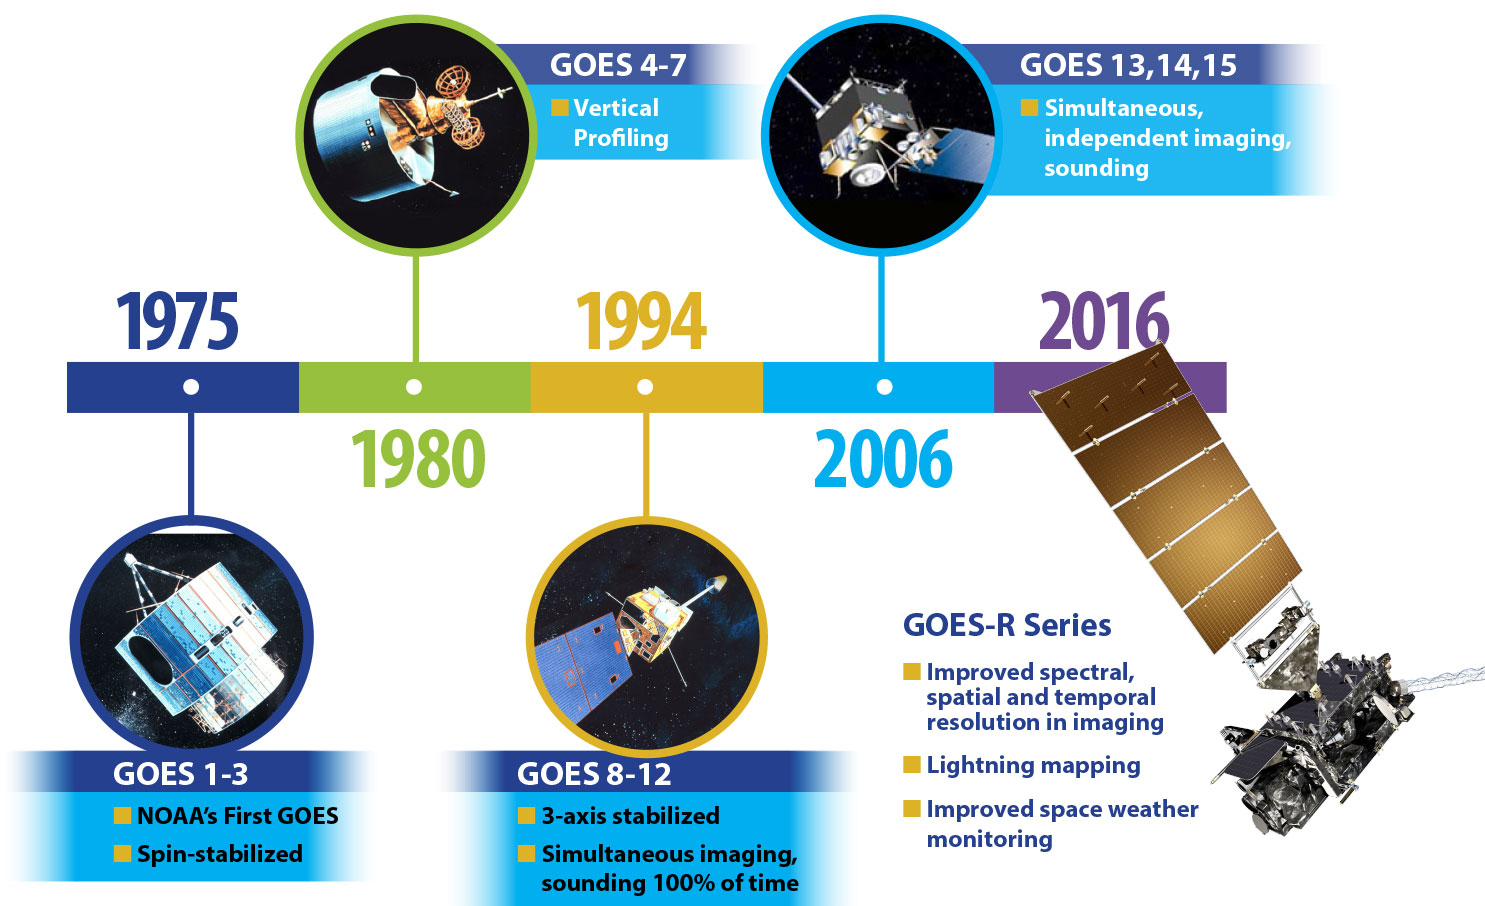
\includegraphics[width=0.7\linewidth]{figs/goes_sat.jpeg}}

\vspace{6mm}



SWPC (\href{{https://www.swpc.noaa.gov/products/goes-x-ray-flux}}{Space Weather Prediction Center}) a utilisé ces données pour produire les ensembles et tracés de données de rayons X moyennés sur 1 minute et 5 minutes.


Le but de cet exercice est de tracer 24 heures, pour un intervalle de mesure d'une minute, des données solaires aux rayons X enregistrées par le satellite GOES. Dans le répertoire courant (répertoire de ce notebook Jupyter), nous avons un dossier \Verb!data_GOES! contenant 12 fichiers dont le nom est formaté comme suit \Verb!YYYYMMDD_Gp_xr_1m.txt! avec:

\begin{itemize}
\item \textbf{YYYY} est l'année de l'enregistrement des données

\item \textbf{MM} estle mois de l'enregistrement des données

\item \textbf{DD} est le jour de l'enregistrement des données

\item \textbf{Gp} est la générartion du satellite GOES (GOES-15)

\item \textbf{1m} résolution de l'enregistrement des données
\end{itemize}

\noindent
\begin{cod}{cbg_gray}\begin{minted}[fontsize=\fontsize{9pt}{9pt},linenos=false,mathescape,baselinestretch=1.0,fontfamily=tt,xleftmargin=2mm]{python}
ls data_GOES/  # Afficher le contenu du dossier data_GOES
\end{minted}
\end{cod}
\noindent

\begin{cod}{cbg_gray}\begin{minted}[fontsize=\fontsize{9pt}{9pt},linenos=false,mathescape,baselinestretch=1.0,fontfamily=tt,xleftmargin=2mm]{text}
20120607_Gp_xr_1m.txt  20120615_Gp_xr_1m.txt  20120627_Gp_xr_1m.txt
20120609_Gp_xr_1m.txt  20120616_Gp_xr_1m.txt  20120628_Gp_xr_1m.txt
20120613_Gp_xr_1m.txt  20120617_Gp_xr_1m.txt  20120629_Gp_xr_1m.txt
20120614_Gp_xr_1m.txt  20120620_Gp_xr_1m.txt  20120630_Gp_xr_1m.txt
\end{minted}
\end{cod}
\noindent



Soit par exemple le fichier \Verb!data_GOES/20120609_Gp_xr_1m.txt! suivant:

\begin{cod}{cbg_gray}\begin{minted}[fontsize=\fontsize{9pt}{9pt},linenos=false,mathescape,baselinestretch=1.0,fontfamily=tt,xleftmargin=2mm]{text}
:Data_list: 20120609_Gp_xr_1m.txt
:Created: 2012 Jun 10 0010 UTC
# Prepared by the U.S. Dept. of Commerce, NOAA, Space Weather Prediction Center
# Please send comments and suggestions to SWPC.Webmaster@noaa.gov
#
# Label: Short = 0.05- 0.4 nanometer
# Label: Long  = 0.1 - 0.8 nanometer
# Units: Short = Watts per meter squared
# Units: Long  = Watts per meter squared
# Source: GOES-15
# Location: W135
# Missing data: -1.00e+05
#
#         1-minute GOES-15 Solar X-ray Flux
#
#                 Modified Seconds
# UTC Date  Time   Julian  of the
# YR MO DA  HHMM    Day     Day       Short       Long
#-------------------------------------------------------
2012 06 09  0000   56087      0     1.62e-08    7.81e-07
2012 06 09  0001   56087     60     1.70e-08    7.92e-07
2012 06 09  0002   56087    120     1.85e-08    8.21e-07
2012 06 09  0003   56087    180     1.90e-08    8.41e-07
2012 06 09  0004   56087    240     1.86e-08    8.50e-07
2012 06 09  0005   56087    300     1.98e-08    8.59e-07
.... .. ..  ....   .....   ....     ........    ........
.... .. ..  ....   .....   ....     ........    ........
.... .. ..  ....   .....   ....     ........    ........
2012 06 09  2352   56087  85920     5.48e-09    5.50e-07
2012 06 09  2353   56087  85980     3.94e-09    5.48e-07
2012 06 09  2354   56087  86040     3.68e-09    5.45e-07
2012 06 09  2355   56087  86100     3.91e-09    5.44e-07
2012 06 09  2356   56087  86160     2.28e-09    5.48e-07
2012 06 09  2357   56087  86220     5.71e-09    5.64e-07
2012 06 09  2358   56087  86280     1.15e-08    5.96e-07
2012 06 09  2359   56087  86340     1.62e-08    6.49e-07
\end{minted}
\end{cod}
\noindent

Dans le même graphique, tracer les tableaux \textbf{Short X-ray} et \textbf{Long X-ray} en fonction de temps \textbf{Universal Time} (Heure de la journée GMT):


\subex{a)}
Définir les tableaux \Verb!Xray_s! et \Verb!Xray_L! qui correspondent au $6^{éme}$ et au $7^{éme}$ colonnes dans le fichier (on compte les colonnes à partir de zéro). Utilisez la fonction \texttt{numpy.loadtxt} comme indiqué dans le cours3 (\href{{https://codetunisia.github.io/CoursSimNum/cours3/md/cours3.html#lecture-de-donn%C3%A9es}}{lecture de données}) et précisez les numéros des colonnes avec l'argument \texttt{usecols}, utilisez le help (\texttt{help(np.loadtxt)}) dans le notebook.


% --- begin solution of exercise ---
\paragraph{Solution.}
Les tableaux \Verb!Xray_s! et \Verb!Xray_L! sont définis de la façon suivante:
\begin{cod}{cbg_gray}\begin{minted}[fontsize=\fontsize{9pt}{9pt},linenos=false,mathescape,baselinestretch=1.0,fontfamily=tt,xleftmargin=2mm]{python}
from pylab import *
NomFichier = "data_GOES/20120609_Gp_xr_1m.txt"
Xray_s,Xray_L = np.loadtxt(NomFichier, skiprows=18, usecols=[6,7],unpack=True)

\end{minted}
\end{cod}
\noindent

% --- end solution of exercise ---

\subex{b)}
Définir le tableau \texttt{temps} en utilisant la fonction \texttt{numpy.arange()} (voir cours3: \href{{https://codetunisia.github.io/CoursSimNum/cours3/md/cours3.html#utilisation-de-fonctions-g%C3%A9n%C3%A9ratrices-de-tableaux-et-de-matrices}}{Utilisation de fonctions génératrices de tableaux et de matrices}).


% --- begin solution of exercise ---
\paragraph{Solution.}
Le tableau temps s'écrit:
\begin{cod}{cbg_gray}\begin{minted}[fontsize=\fontsize{9pt}{9pt},linenos=false,mathescape,baselinestretch=1.0,fontfamily=tt,xleftmargin=2mm]{python}
temps = np.arange(0.0, 24.0 , 24.0/len(Xray_L))
\end{minted}
\end{cod}
\noindent

% --- end solution of exercise ---

\subex{c)}
Tracer \Verb!Xray_s! et \Verb!Xray_L! en fonction de \texttt{temps} afin de reproduire le graphique suivant (voirs cours3: \href{{https://codetunisia.github.io/CoursSimNum/cours3/md/cours3.html#trac%C3%A9s-logarithmiques}}{Tracés logarithmiques}):


\vspace{6mm}

% inline figure
\centerline{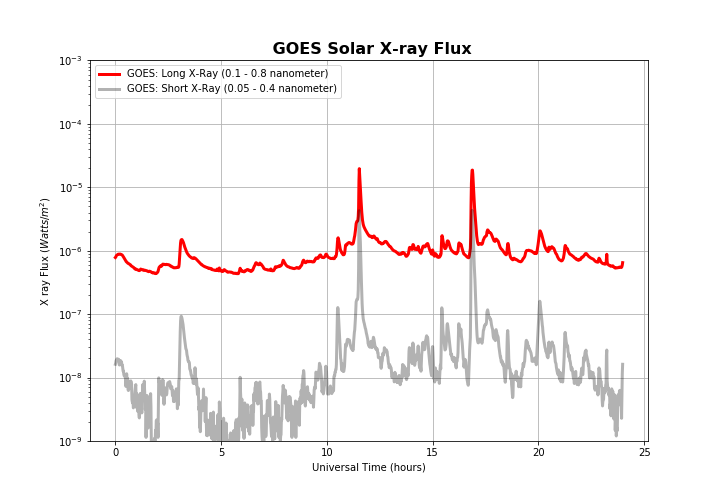
\includegraphics[width=0.7\linewidth]{figs/goes_plot.png}}

\vspace{6mm}




% --- begin solution of exercise ---
\paragraph{Solution.}
\begin{cod}{cbg_gray}\begin{minted}[fontsize=\fontsize{9pt}{9pt},linenos=false,mathescape,baselinestretch=1.0,fontfamily=tt,xleftmargin=2mm]{python}
plt.figure(figsize=(10, 7))
plt.semilogy(temps, Xray_L,color='r',linewidth=3,label="GOES: Long X-Ray (0.1 - 0.8 nanometer)")
plt.semilogy(temps, Xray_s,color='k',linewidth=3,label="GOES: Short X-Ray (0.05 - 0.4 nanometer)", alpha=.3)
plt.title(" GOES Solar X-ray Flux", fontsize=16, weight="bold" )
plt.ylabel("X ray Flux ($Watts/m^2$)"); plt.xlabel("Universal Time (hours)")
plt.legend(loc='upper left')
plt.ylim(1e-9, 1e-3)
plt.grid()

savefig("goes_plot.png")
plt.show()
\end{minted}
\end{cod}
\noindent

% --- end solution of exercise ---

\end{doconceexercise}
% --- end exercise ---




% --- begin exercise ---
\begin{doconceexercise}
\refstepcounter{doconceexercisecounter}

\exercisesection{Exercise \thedoconceexercisecounter: Fonctions spéciales (intégrales de Fresnel et spirale de Cornu)}


Les intégrales de Fresnel ont été introduites par le physicien français Augustin Fresnel (1788-1827) lors de ses travaux sur les interférences lumineuses (voici un article intéressant à lire: \href{{http://www.mathouriste.eu/Fresnel/Fresnel.html}}{Fresnel, des Mathématiques en Lumière}).

Ces intégrales doivent être calculées numériquement à partir des développements en série des intégrales:

$$\int_{0}^{x} e^{-i\frac{\pi t^{2}}{2}} dt = \int_{0}^{x} cos(t^2) dt -i \int_{0}^{x} sin(t^2) dt= C(x) -i S(x)$$

Les fonctions de Fresnel sont des fonctions spéciales, définies par:

Pour $x \geq \sqrt{\frac{8}{\pi}}$
\begin{equation*}
\begin{aligned}
C(x) &= \frac{1}{2} + \cos\left(\frac{\pi x^{2}}{2}\right) gg1 + \sin\left(\frac{\pi x^{2}}{2}\right) ff1\\
S(x) &=  \frac{1}{2} - \cos\left(\frac{\pi x^{2}}{2}\right) ff1 + \sin\left(\frac{\pi x^{2}}{2}\right) gg1
\end{aligned}
\end{equation*}
et pour $0 \leq x < \sqrt{\frac{8}{\pi}}$
\begin{equation*}
\begin{aligned}
C(x) &= \cos\left(\frac{\pi x^{2}}{2}\right) gg2 + \sin\left(\frac{\pi x^{2}}{2}\right) ff2 \\
S(x) &= - \cos\left(\frac{\pi x^{2}}{2}\right) ff2 + \sin\left(\frac{\pi x^{2}}{2}\right) gg2
\end{aligned}
\end{equation*}
Où:
\begin{equation*}
\begin{aligned}
ff1 = \sum\limits_{n=0}^{11} \frac{d_{n}}{x^{2n+1}}\left(\frac{8}{\pi}\right)^{n+1/2} & gg1 = \sum\limits_{n=0}^{11} \frac{c_{n}}{x^{2n+1}}\left(\frac{8}{\pi}\right)^{n+1/2}\\
ff2 = \sum\limits_{n=0}^{11} b_{n}x^{2n+1}\left(\frac{\pi}{8}\right)^{n+1/2} & gg2 = \sum\limits_{n=0}^{11} a_{n}x^{2n+1}\left(\frac{\pi}{8}\right)^{n+1/2}
\end{aligned}
\end{equation*}
et $a_n$, $b_n$, $c_n$ et $d_n$ sont des coefficients tabulés  (\href{{https://www.ams.org/journals/mcom/1960-14-072/S0025-5718-1960-0121973-3/S0025-5718-1960-0121973-3.pdf}}{*J.Boersma Math Computation 14,380(1960)*}) et donnés dans un fichier \textbf{coef.dat} dans le répertoire de ce notebook:

\begin{cod}{cbg_gray}\begin{minted}[fontsize=\fontsize{9pt}{9pt},linenos=false,mathescape,baselinestretch=1.0,fontfamily=tt,xleftmargin=2mm]{text}
#--------------------------------------------------
#    an            bn          cn           dn
#--------------------------------------------------
+1.595769140 -0.000000033 -0.000000000 +0.199471140
-0.000001702 +4.255387524 -0.024933975 +0.000000023
-6.808568854 -0.000092810 +0.000003936 -0.009351341
-0.000576361 -7.780020400 +0.005770956 +0.000023006
+6.920691902 -0.009520895 +0.000689892 +0.004851466
-0.016898657 +5.075161298 -0.009497136 +0.001903218
-3.050485660 -0.138341947 +0.011948809 -0.017122914
-0.075752419 -1.363729124 -0.006748873 +0.029064067
+0.850663781 -0.403349276 +0.000246420 -0.027928955
-0.025639041 +0.702222016 +0.002102967 +0.016497308
-0.150230960 -0.216195929 -0.001217930 -0.005598515
+0.034404779 +0.019547031 +0.000233939 +0.000838386
\end{minted}
\end{cod}
\noindent


Écrire un programme Python qui calcule les fonctions de Fresnel $C(x)$ et $S(x)$ ainsi que leurs représentations graphiques:


\subex{a)}
Définir les fonctions \texttt{ff1(x)}, \texttt{gg1(x)}, \texttt{ff2(x)} et \texttt{gg2(x)}. Chaque fonction renvoie la valeur de la somme qui lui correspond.


% --- begin solution of exercise ---
\paragraph{Solution.}
Les fonctions \texttt{ff1(x)}, \texttt{gg1(x)}, \texttt{ff2(x)} et \texttt{gg2(x)} sont les suivantes:
\begin{cod}{cbg_gray}\begin{minted}[fontsize=\fontsize{9pt}{9pt},linenos=false,mathescape,baselinestretch=1.0,fontfamily=tt,xleftmargin=2mm]{python}
from pylab import *

def ff1(x):
    S = 0
    for i in range(12):
        fn = (8 / pi)**(i + 0.5) * dn[i]
        S += fn * x**(-2 * i - 1)
    return S

def gg1(x):
    S = 0
    for i in range(12):
        gn = (8 / pi)**(i + 0.5) * cn[i]
        S += gn * x**(-2 * i - 1)
    return S

def ff2(x):
    S = 0
    for i in range(12):
        fn = (pi / 8)**(i + 0.5) * bn[i]
        S += fn * x**(2 * i + 1)
    return S

def gg2(x):

    S = 0
    for i in range(12):
        gn = (pi/8)**(i + 0.5) * an[i]
        S +=  gn * x**(2 * i + 1)
    return S
\end{minted}
\end{cod}
\noindent

% --- end solution of exercise ---

\subex{b)}
Définir les fonctions Python \texttt{C(x)} et \texttt{S(x)} qui renvoient respectivement les listes, les valeurs de $C(x)$ et $S(x)$, \texttt{CF} et` SF` (en utilisant une boucle \texttt{for} pour remplir les listes par exemple).


% --- begin solution of exercise ---
\paragraph{Solution.}
Les fonctions Python \texttt{C(x)} et \texttt{S(x)} sont les suivantes:

\begin{cod}{cbg_gray}\begin{minted}[fontsize=\fontsize{9pt}{9pt},linenos=false,mathescape,baselinestretch=1.0,fontfamily=tt,xleftmargin=2mm]{python}
def C(x):
    CF=[]
    for i in range(len(x)):
        if x[i] >= sqrt(8/pi):
            cf=0.5 + cos((pi*x[i]**2)/2)*gg1(x[i]) + sin((pi*x[i]**2)/2)*ff1(x[i])
            CF.append(cf)
        elif 0 <= x[i] < sqrt(8/pi):
            cf = cos((pi*x[i]**2)/2)*gg2(x[i]) + sin((pi*x[i]**2)/2)*ff2(x[i])
            CF.append(cf)
    return CF
def S(x):
    SF=[]
    for i in range(len(x)):
        if x[i] >= sqrt(8/pi):
            sf = 0.5 - cos((pi*x[i]**2)/2)*ff1(x[i]) + sin((pi*x[i]**2)/2)*gg1(x[i])
            SF.append(sf)
        elif 0 <= x[i] < sqrt(8/pi):
            sf = -cos((pi*x[i]**2)/2)*ff2(x[i]) + sin((pi*x[i]**2)/2)*gg2(x[i])
            SF.append(sf)
    return SF
\end{minted}
\end{cod}
\noindent

% --- end solution of exercise ---

\subex{c)}
Créer des tableaux \texttt{an}, \texttt{bn}, \texttt{cn} et \texttt{dn} à partir du fichier \textbf{coef.dat}.


% --- begin solution of exercise ---
\paragraph{Solution.}
Les tableaux \texttt{an}, \texttt{bn}, \texttt{cn} et \texttt{dn} sont chargés  à partir du fichier \textbf{coef.dat} à l'aide del a fonction \texttt{numpy.loadtxt()}:
\begin{cod}{cbg_gray}\begin{minted}[fontsize=\fontsize{9pt}{9pt},linenos=false,mathescape,baselinestretch=1.0,fontfamily=tt,xleftmargin=2mm]{python}
an, bn, cn, dn = loadtxt('coef.dat', comments='#', usecols=(0, 1, 2, 3), unpack=True)
\end{minted}
\end{cod}
\noindent

% --- end solution of exercise ---

\subex{d)}
Créer un tableau \texttt{x}. Utilisez 800 intervalles pour évaluer les points dans [0,10] (cas où $x \geq 0$).


% --- begin solution of exercise ---
\paragraph{Solution.}
Le tableau \texttt{x} s'écrit:
\begin{cod}{cbg_gray}\begin{minted}[fontsize=\fontsize{9pt}{9pt},linenos=false,mathescape,baselinestretch=1.0,fontfamily=tt,xleftmargin=2mm]{python}
x = linspace(0,10, 500)
\end{minted}
\end{cod}
\noindent

% --- end solution of exercise ---

\subex{e)}
Transformer \texttt{C(x)} et \texttt{S(x)} en tableaux \texttt{numpy}, respectivement \texttt{CF} et \texttt{SF}.


% --- begin solution of exercise ---
\paragraph{Solution.}
Les listes \texttt{C(x)} et \texttt{S(x)} sont transformés en tableaux \texttt{numpy} à l'aide de la fonction \texttt{numpy.array()}:
\begin{cod}{cbg_gray}\begin{minted}[fontsize=\fontsize{9pt}{9pt},linenos=false,mathescape,baselinestretch=1.0,fontfamily=tt,xleftmargin=2mm]{python}
CF = array(C(x)); SF = array(S(x))
\end{minted}
\end{cod}
\noindent

% --- end solution of exercise ---

\subex{f)}
Tracer une grille de figures à 2 colonnes (voir Cours3: \href{{https://codetunisia.github.io/CoursSimNum/cours3/md/cours3.html#linstruction-subplot}}{Vues en grille}) dont le graphique de gauche représente \texttt{CF} et \texttt{SF} en fonction de \texttt{x} et le graphique de droite représente une \href{{https://fr.wikipedia.org/wiki/Clotho%C3%AFde}}{clothoïde} (ou spirale de Cornu, ou Spirale de Fresnel..)`SF` en fonction de \texttt{CF}.
La sortie de ce programme devrait être comme suit:


\vspace{6mm}

% inline figure
\centerline{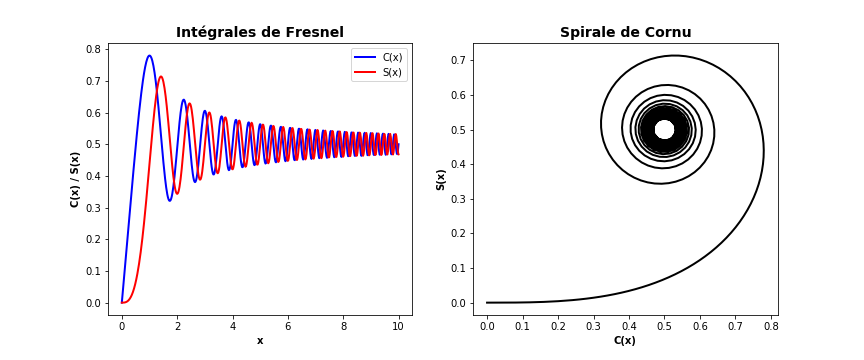
\includegraphics[width=0.7\linewidth]{figs/fresnel.png}}

\vspace{6mm}




% --- begin solution of exercise ---
\paragraph{Solution.}
La représentation graphique des intégrales de Fresnel et du spirale de Cornu est donc:
\begin{cod}{cbg_gray}\begin{minted}[fontsize=\fontsize{9pt}{9pt},linenos=false,mathescape,baselinestretch=1.0,fontfamily=tt,xleftmargin=2mm]{python}
plt.figure(figsize=(12,5))
subplot(1,2,1)
plt.plot(x, CF,'b', x, SF,'r', linewidth=2)
plt.xlabel("x", fontweight='bold'); plt.ylabel("C(x) / S(x)", fontweight='bold')
plt.title("Intégrales de Fresnel", fontsize=14, fontweight='bold')
plt.legend(["C(x)","S(x)"])
subplot(1,2,2)
plt.plot(CF, SF, linewidth = 2, color = 'k')
plt.xlabel("C(x)", fontweight='bold'); plt.ylabel("S(x)", fontweight='bold')
plt.title("Spirale de Cornu", fontsize=14, fontweight='bold')

plt.savefig("fresnel.png")
plt.show()
\end{minted}
\end{cod}
\noindent

% --- end solution of exercise ---

\end{doconceexercise}
% --- end exercise ---


% ------------------- end of main content ---------------

% #ifdef PREAMBLE
\end{document}
% #endif

